\documentclass{beamer}
\usetheme{metropolis}           % Use metropolis theme
\title{Les nombres à virgule flottante}
\subtitle{à l'arrondi près}
\date{\today}
\definecolor{DarkOrange}{RGB}{255, 64, 0}
\definecolor{SignColor}{RGB}{51, 204, 255}
\definecolor{ExponentColor}{RGB}{0, 255, 153}
\definecolor{FractionColor}{RGB}{255, 102, 102}

\setbeamercolor{frametitle}{bg=DarkOrange}
\usepackage{graphicx}
\usepackage{anyfontsize}
\usepackage{listings}
\usepackage{xcolor}
\graphicspath{ {./images/} }

\begin{document}
  \maketitle
  \begin{frame}{IEEE-754 (1985)}
Définit :
    \begin{itemize}
      \item des représentations : simple précision (binary32), double précision (binary64) et étendus (40 et 80 bits)
      \item des valeurs spéciales : $+\infty$, $-\infty$, -0.0, NaNs
      \item des opérations : +, -, / , *, $\sqrt{x}$, comparaisons, floating point remainder, arrondi à l'entier
      \item des arrondis pour les affectations et opérations : au pair le plus proche, opposé à zéro, vers zéro, vers $+\infty$ et vers $-\infty$
    \end{itemize}
  \end{frame}
  
  \begin{frame}{IEEE-754}
    Implémentation matérielle (FPU) : 
    \begin{itemize}
      \item Rapidité (1 cycle pour certaines opérations)
      \item Délégation/respect de la norme (presque tout le temps, Pentium FDIV bug)
    \end{itemize}
  \end{frame}
  
  \begin{frame}{Comment représenter un nombre à virgule} 
    $+0.15625 = +(0*10^{0} + 1*10^{-1} + 5*10^{-2} + 6*10^{-3} + 2*10^{-4} + 5*10^{-5})$
    \begin{center}
      \begin{tabular}{|c|c|c|c|c|c|c|c|c|c|} \hline
        ... & $10^{1}$ & $10^{0}$ & $10^{-1}$ & $10^{-2}$ & $10^{-3}$ & $10^{-4}$ & $10^{-5}$ & $10^{-6}$ & ... \\ \hline
        0 & 0 & 0 & 1 & 5 & 6 & 2 & 5 & 0 & 0\\ \hline
      \end{tabular}
    \end{center}
  \end{frame}
  
  \begin{frame}{Comment représenter un nombre à virgule} 
    \begin{center}
\fontsize{100}{110}\selectfont 0 \hspace{1cm} 1
    \end{center}
  \end{frame}
  
  \begin{frame}{Comment représenter un nombre à virgule} 
    $+0.15625 = +(0*2^{0} + 0*2^{-1} + 0*2^{-2} + $\textcolor{DarkOrange}{$1*2^{-3}$} $+ 0*2^{-4} + $\textcolor{DarkOrange}{$1*2^{-5}$})
    \begin{center}
      \begin{tabular}{|c|c|c|c|c||c|c|c|c|c|} \hline
        ... & $2^{1}$ & $2^{0}$ & $2^{-1}$ & $2^{-2}$ & $2^{-3}$ & $2^{-4}$ & $2^{-5}$ & $2^{-6}$ & ... \\ \hline
        0 & 0 & 0 & 0 & 0 & \textcolor{DarkOrange}{1} & 0 & \textcolor{DarkOrange}{1} & 0 & 0 \\ \hline
      \end{tabular}
    \end{center}
  \end{frame}
  
  \begin{frame}{Comment représenter un nombre à virgule} 
    \begin{Huge}
    \begin{center}
    +0.15625
    \end{center}
    \end{Huge}
Pour résumer, on a besoin : 
    \begin{itemize}
      \item d'un signe : + 
      \item d'un décalage : -3 
      \item d'une charge : 0b 101
    \end{itemize}
  \end{frame}
 
  \begin{frame}{Comment représenter un nombre à virgule} 
    \begin{Huge}
    \begin{center}
    +0.15625
    \end{center}
    \end{Huge}
Pour résumer, on a besoin : 
    \begin{itemize}
      \item d'un signe : + $\Rightarrow$ signe
      \item d'un décalage : -3 $\Rightarrow$ exposant (biaisé pour éviter le signe)
      \item d'une charge : 0b 101 $\Rightarrow$ mantisse (tronquée pour gagner un bit sauf dénormalisé)
    \end{itemize}
    
    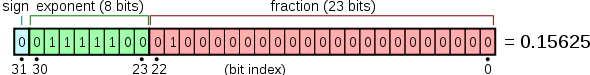
\includegraphics[width=\textwidth]{float_representation}
  \end{frame}
  
  \begin{frame}{Problème 1/N} 
    \begin{center}
      \fontsize{100}{110}\selectfont $\pi$ 
    \end{center}
  \end{frame}
  
  \begin{frame}{Problème 1/N} 
    \begin{center}
      \fontsize{100}{110}\selectfont $\pi$ 
    \end{center}
    \begin{center}
      3.14159265358979323846264338327950288419716939937510582097494459230
    \end{center}
  \end{frame}
  
  \begin{frame}{Problème 1/N} 
    \begin{center}
      \fontsize{100}{110}\selectfont $1/3$
    \end{center}
  \end{frame}
  
  \begin{frame}{Problème 1/N} 
    \begin{center}
      \fontsize{100}{110}\selectfont $1/3$
    \end{center}
    \begin{center}
      0.33333333333333333333333333333333333333333333333333333333333333333
    \end{center}
  \end{frame}
  
    \begin{frame}{Problème 1/N} 
    \begin{center}
      \fontsize{100}{110}\selectfont{$0.4$}
    \end{center}
  \end{frame}
  
  \begin{frame}{Problème 1/N} 
    \begin{center}
      \fontsize{100}{110}\selectfont{$0.4$}
    \end{center}
    \begin{center}
      0.4
    \end{center}
  \end{frame}
  
  \begin{frame}{Problème 1/N} 
    \begin{center}
      \fontsize{100}{110}\selectfont{$0.4$}
    \end{center}
    \begin{center}
      0b \textcolor{SignColor}{0} \textcolor{ExponentColor}{01111101} \textcolor{FractionColor}{10011001100110011001101}
    \end{center}
  \end{frame}
  
  \begin{frame}{Problème 1/N} 
    \begin{center}
      \fontsize{100}{110}\selectfont{$0.4$}
    \end{center}
    \begin{center}
      0b \textcolor{SignColor}{0} \textcolor{ExponentColor}{01111101} \textcolor{FractionColor}{10011001100110011001101} $\approx$ 0.4
    \end{center}
  \end{frame}
  
  \begin{frame}{Problème 1/N} 
    \begin{center}
      \fontsize{100}{110}\selectfont $0.4$
    \end{center}
    \begin{center}
      0b \textcolor{SignColor}{0} \textcolor{ExponentColor}{01111101} \textcolor{FractionColor}{10011001100110011001101} \fontsize{40}{50}\selectfont{$\approx$} 0.4
    \end{center}
  \end{frame}
  
  \begin{frame}{Problème 1/N} 
    \begin{center}
      \fontsize{70}{80}\selectfont $0.4\approx0.4$
    \end{center}
  \end{frame}
  
  \begin{frame}{Problème 1/N} 
    \begin{center}
      \fontsize{50}{60}\selectfont Des questions ?
    \end{center}
  \end{frame}
  
  \begin{frame}{Problème 1/N} 
    \begin{center}
      \Large 0b \textcolor{SignColor}{0} \textcolor{ExponentColor}{01111101} \textcolor{FractionColor}{10011001100110011001101} \\
      = \\
      0.4000000059604644775390625
    \end{center}
    \begin{center}
    Précision à revoir ... \\
    (spoiler alert : c'est pareil en double précision)
    \end{center}
  \end{frame}
 
  \begin{frame}{Simple vs Double} 
    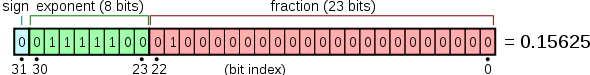
\includegraphics[width=\textwidth]{float_representation}
    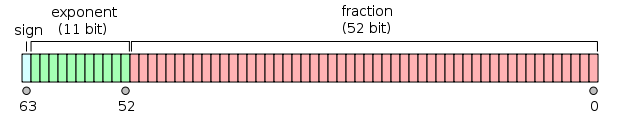
\includegraphics[width=\textwidth]{double_representation}
          \vfill{}
          \begin{tiny}
    By Vectorization: Stannered - Own work based on: Float example.PNG, CC BY-SA 3.0, https://commons.wikimedia.org/w/index.php?curid=3357169
          \end{tiny}
  \end{frame}
  
    \begin{frame}{Problème 2/N}
    IEEE-754 : Taille mémoire figée (32 ou 64 bits) \\
    \textcolor{white}{ } \\
    \textcolor{white}{ } \\
   \end{frame}
  
  \begin{frame}{Problème 2/N}
    IEEE-754 : Taille mémoire figée (32 ou 64 bits) \\
    $\Rightarrow$ Nombre fini de permutations ($\sim$ $2^{32}$ ou $2^{64}$ possibilités)\\
    \textcolor{white}{ } \\
  \end{frame}
  
  \begin{frame}{Problème 2/N}
    IEEE-754 : Taille mémoire figée (32 ou 64 bits) \\
    $\Rightarrow$ Nombre fini de permutations ($\sim$ $2^{32}$ ou $2^{64}$ possibilités)\\
    $\Rightarrow$ Précision et représentation limitées \\
  \end{frame}
  
  \begin{frame}{Problème 2/N}
Pour un float :
\begin{itemize}
\item la plus grande valeur représentable est : 
\begin{itemize}
\item 0b \textcolor{SignColor}{0} \textcolor{ExponentColor}{11111111} \textcolor{FractionColor}{11111111111111111111111}
\item 
\end{itemize}
\item la plus petite valeur représentable (hors 0) est : 
\begin{itemize}
\item 0b \textcolor{SignColor}{0} \textcolor{ExponentColor}{00000000} \textcolor{FractionColor}{00000000000000000000001}
\item 
\end{itemize}
\end{itemize}
\bigbreak
\begin{huge}
\textcolor{white}{ }
\end{huge}
  \end{frame}
    
  \begin{frame}{Problème 2/N}
Pour un float :
\begin{itemize}
\item la plus grande valeur représentable est : 
\begin{itemize}
\item 0b \textcolor{SignColor}{0} \textcolor{ExponentColor}{11111111} \textcolor{FractionColor}{11111111111111111111111}
\item NaN
\end{itemize}
\item la plus petite valeur représentable (hors 0) est : 
\begin{itemize}
\item 0b \textcolor{SignColor}{0} \textcolor{ExponentColor}{00000000} \textcolor{FractionColor}{00000000000000000000001}
\item $1.17549435*10^{-38}$
\end{itemize}
\end{itemize}
\bigbreak
\begin{huge}
\textcolor{white}{ }
\end{huge} 
  \end{frame}
    
  \begin{frame}{Problème 2/N}
Pour un float :
\begin{itemize}
\item la plus grande valeur représentable est : 
\begin{itemize}
\item 0b \textcolor{SignColor}{0} \textcolor{ExponentColor}{11111110} \textcolor{FractionColor}{11111111111111111111111}
\item $3.40282346639*10^{38}$
\end{itemize}
\item la plus petite valeur représentable (hors 0) est : 
\begin{itemize}
\item 0b \textcolor{SignColor}{0} \textcolor{ExponentColor}{00000000} \textcolor{FractionColor}{00000000000000000000001}
\item $1.40129846432*10^{-45}$ (dénormalisé)
\end{itemize}
\end{itemize}
\bigbreak
\begin{huge}
\textcolor{white}{ }
\end{huge}
  \end{frame}
  
  \begin{frame}{Problème 2/N}
Pour un float :
\begin{itemize}
\item la plus grande valeur représentable est : 
\begin{itemize}
\item 0b \textcolor{SignColor}{0} \textcolor{ExponentColor}{11111110} \textcolor{FractionColor}{11111111111111111111111}
\item $3.40282346639*10^{38}$
\end{itemize}
\item la plus petite valeur représentable (hors 0) est : 
\begin{itemize}
\item 0b \textcolor{SignColor}{0} \textcolor{ExponentColor}{00000000} \textcolor{FractionColor}{00000000000000000000001}
\item $1.40129846432*10^{-45}$ (dénormalisé)
\end{itemize}
\end{itemize}
\bigbreak
\begin{Large}
$\Rightarrow 10^{38} / 10^{-45} = 10^{83}$ valeurs possibles théoriques
\end{Large}
  \end{frame}
  
  \begin{frame}{Problème 2/N} 
  Pour rappel (et schématiser) avec des floats :
  \begin{itemize}
  \item Nombre de permutations : $2^{32} \approx 4.2*10^{9}$
  \item Nombre de valeurs possibles théoriques : $10^{84}$
  \end{itemize}
        \bigbreak
\begin{huge}
\textcolor{white}{ }
\end{huge}
  \end{frame}
  
    \begin{frame}{Problème 2/N} 
  Pour rappel (et schématiser) avec des floats :
  \begin{itemize}
  \item Nombre de permutations : $2^{32} \approx 4.2*10^{9}$
  \item Nombre de valeurs possibles théoriques : $10^{84}$
  \end{itemize}
            \bigbreak
\begin{huge}
$\Rightarrow$ Le compte n'est pas bon !
\end{huge}
  \end{frame}

      \begin{frame}{Problème 2/N} 
Sorte de fenêtre de précision  : 
\begin{itemize}
\item X chiffres significatifs par rapport à l'exposant (6-7 pour float)
\item précision liée à l'exposant (trade-off magnitude/précision)
\end{itemize}
  \end{frame}
  
    \begin{frame}{Problème 2/N} 
    \begin{center}
      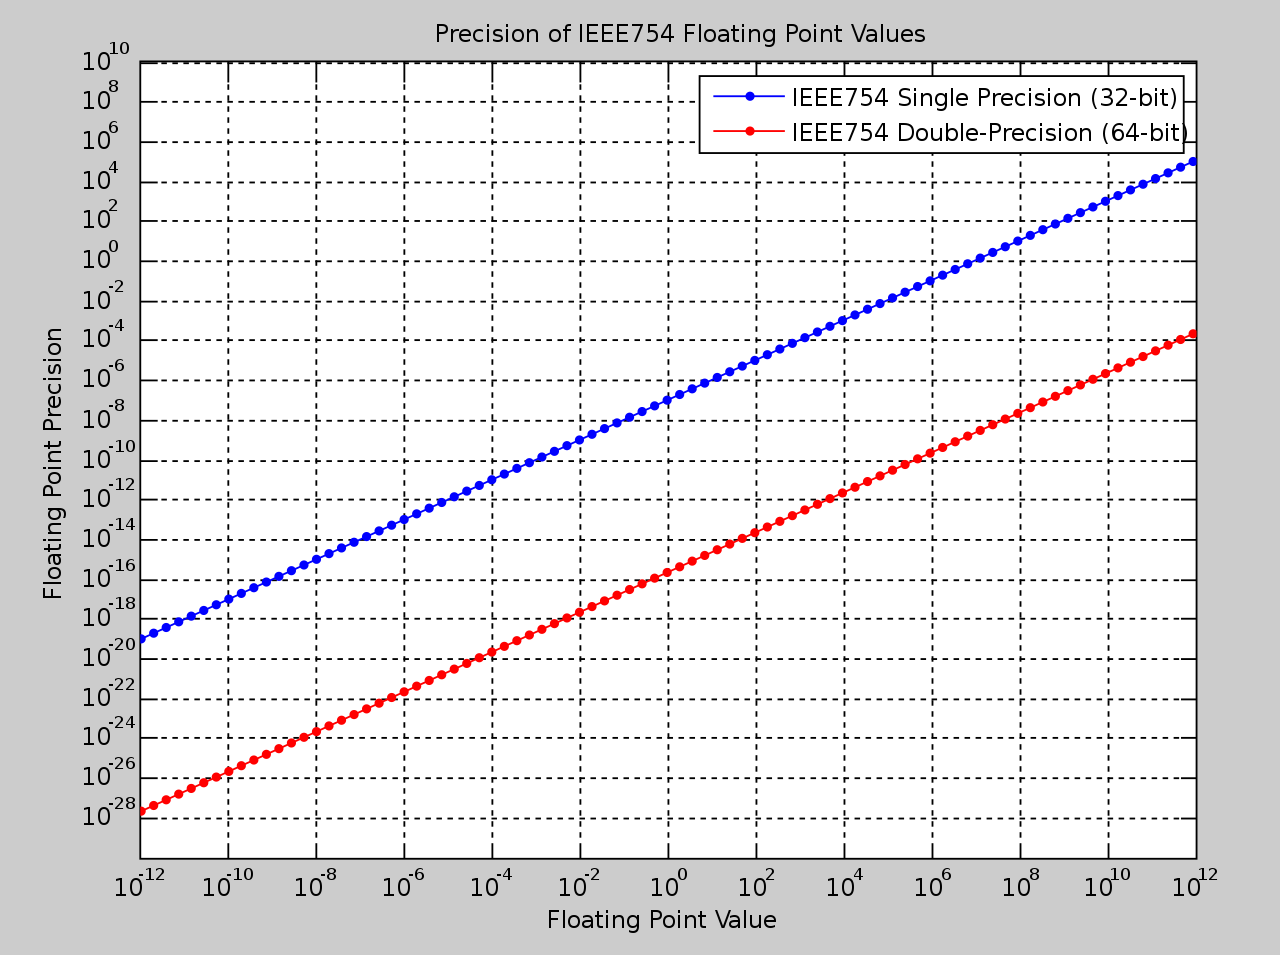
\includegraphics[width=0.7\textwidth]{precision}
      \vfill{}
      \begin{tiny}
By Vectorization: OmenBreeze - Own work based on: IEEE754.png by Ghennessey, CC BY-SA 4.0, https://commons.wikimedia.org/w/index.php?curid=87066073
      \end{tiny}
      \end{center}
  \end{frame}


\defverbatim[colored]\sample{
\begin{lstlisting}[language=C++,basicstyle=\ttfamily,keywordstyle=\color{blue}]
  float m = 20'000'000.0;
  float not_m = 0.0;
  for (int i = 0; i < 20'000'000; ++i) {
    not_m += 1.0;
  }
  std::cout.precision(10);
  std::cout << m << '\n';
  std::cout << not_m << '\n';
\end{lstlisting}
}

\begin{frame}{Problème 2/N} 
\sample
\end{frame}

\defverbatim[colored]\samplewithresult{
\begin{lstlisting}[language=C++,basicstyle=\ttfamily,keywordstyle=\color{blue}]
  float m = 20'000'000.0;
  float not_m = 0.0;
  for (int i = 0; i < 20'000'000; ++i) {
    not_m += 1.0;
  }
  std::cout.precision(10);
  std::cout << m << '\n'; // 20000000
  std::cout << not_m << '\n'; // 16777216
\end{lstlisting}
}  
  
\begin{frame}{Problème 2/N} 
\samplewithresult
\end{frame}

\begin{frame}{Problème 3/N} 
Limite de représentation $\Rightarrow$ quels comportements aux limites et au-delà des limites ? 
\begin{itemize}
\item perte de valeur
\item overflow et underflow
\item annulation
\end{itemize}
\end{frame}

    \begin{frame}{Problème 3/N} 
    \begin{center}
      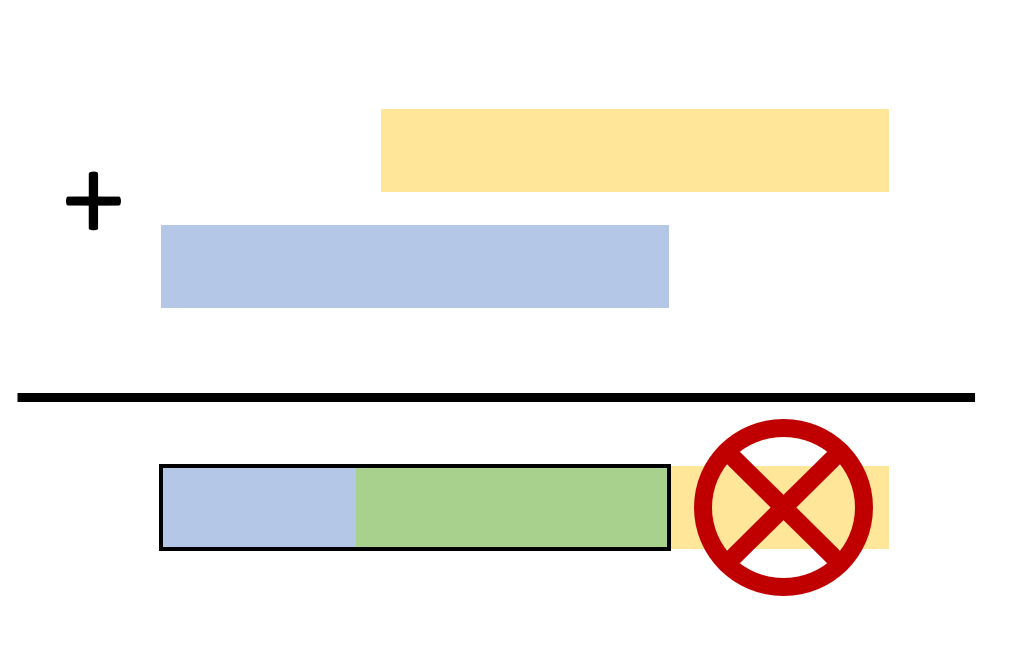
\includegraphics[width=\textwidth]{addition}
      \end{center}
  \end{frame}

    \begin{frame}{Problème 3/N} 
    \begin{center}
      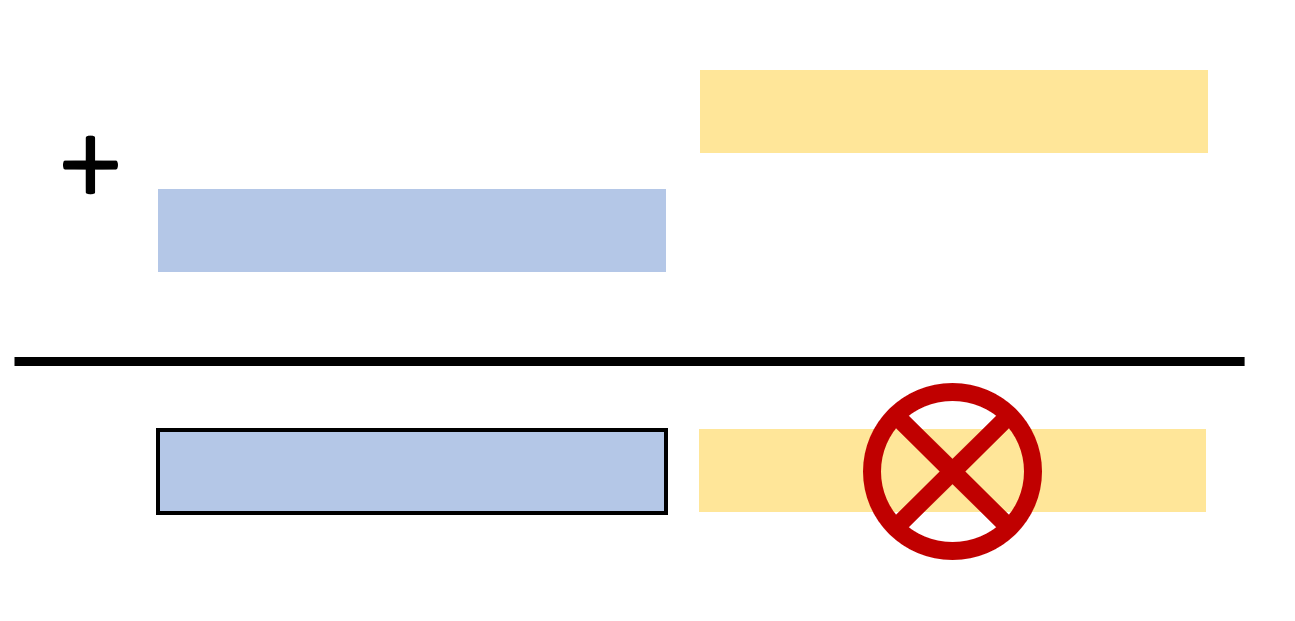
\includegraphics[width=\textwidth]{addition_underflow}
      \end{center}
  \end{frame}

    \begin{frame}{Problème 3/N} 
    \begin{center}
      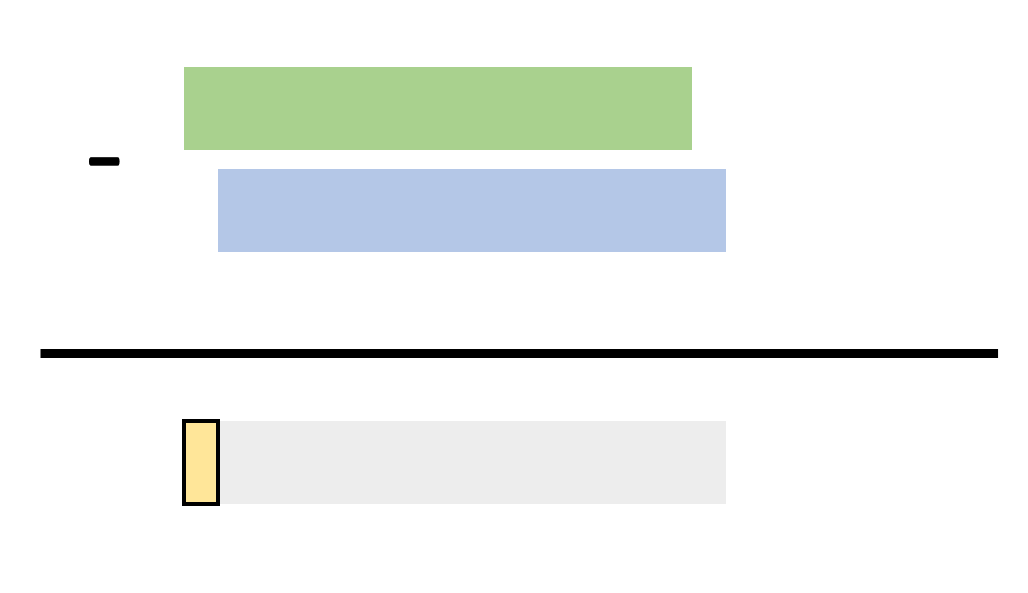
\includegraphics[width=\textwidth]{substraction}
      \end{center}
  \end{frame}

    \begin{frame}{Problème 3/N} 
    \begin{center}
      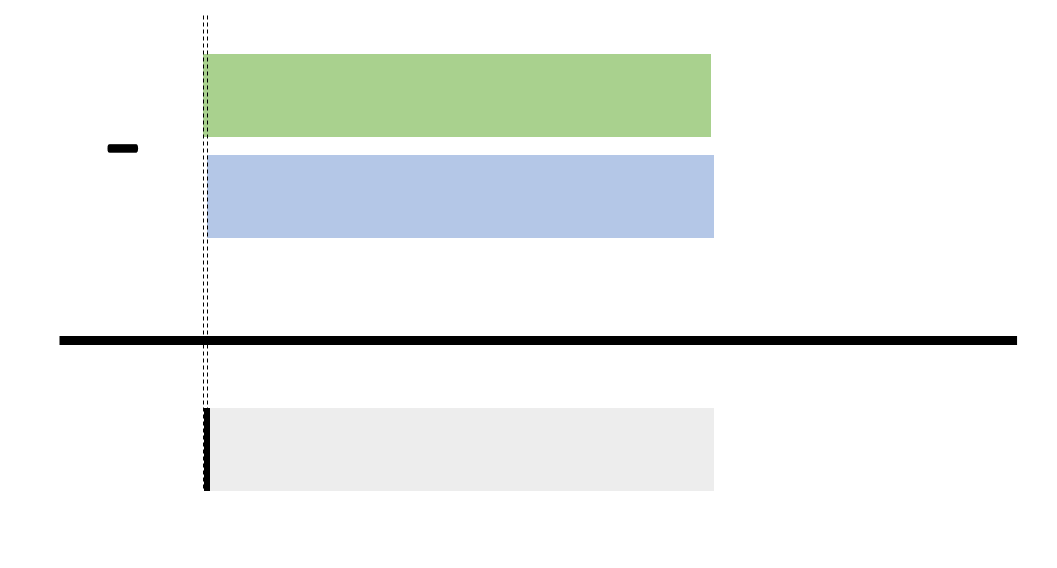
\includegraphics[width=\textwidth]{substraction_cancellation}
      \end{center}
  \end{frame}

    \begin{frame}{Problème 3/N} 
    \begin{center}
    Un (tout petit) peu de mathématiques : \\
      $f(x) = \frac{1}{1-\sqrt{1-x^{2}}}$ \\
      \textcolor{white}{ } \\
      Mathématiquement : $x \neq 0 \Rightarrow f(x)$ valide (pas de division par 0) \\
      \textcolor{white}{ } \\
      \textcolor{white}{ } \\
     \end{center}
  \end{frame}

    \begin{frame}{Problème 3/N} 
    \begin{center}
    Un (tout petit) peu de mathématiques : \\
      $f(x) = \frac{1}{1-\sqrt{1-x^{2}}}$ \\
      \textcolor{white}{ } \\
      Mathématiquement : $x \neq 0 \Rightarrow f(x)$ valide (pas de division par 0) \\
      \textcolor{white}{ } \\
      Informatiquement : $\sqrt{x} < 1.10^{8} \Rightarrow f(x) = Inf$
     \end{center}
  \end{frame}
  
\defverbatim[colored]\randomassociativity{
\begin{lstlisting}[language=C++,basicstyle=\ttfamily,keywordstyle=\color{blue}]
float a, b, c;
int success_counter = 0;
for (auto i = 0; i < 500; ++i) {
  a = dist_a(gen);
  b = dist_b(gen);
  c = dist_c(gen);
  float r1 = (a + b) + c;
  float r2 = a + (b + c);
  if (r1 == r2) {
    ++success_counter;
  }
}
// entre 300 et 400 succes en moyenne
\end{lstlisting}
}  
  
  \begin{frame}{Problème 4/N} 
  \begin{center}
  $(a+b)+c \neq a+(b+c)$ \\
  \end{center}
  \end{frame}
  
  \begin{frame}{Problème 4/N} 
  \randomassociativity
  \end{frame}
  
    \begin{frame}{Problème 4/N} 
    \begin{itemize}
\item a = 9.195287704 \\
\item b = 73.53369141 \\
\item c = 115.2905426 \\
\item (a + b) + c = 198.0195312 \\
\item a + (b + c) = 198.0195160 \\
\item 198.0195312 $\Rightarrow$ 0b \textcolor{SignColor}{0} \textcolor{ExponentColor}{10000110} \textcolor{FractionColor}{10001100000010100000000}\\
\item 198.0195160 $\Rightarrow$ 0b \textcolor{SignColor}{0} \textcolor{ExponentColor}{10000110} \textcolor{FractionColor}{10001100000010011111111}
\end{itemize}
    \end{frame}
    
  \begin{frame}{Problème X/N}
  Parmi les autres problèmes et complexités: 
  \begin{itemize}
  \item opérations complexes ($\sqrt{x}, exp(x), log(x), ...$) faite de manière algorithmiques
  \item implémentation matérielle produisant des résultats différents ou erronés (Pentium FDIV bug)
  \item IEEE-754:2008 qui introduit de nouveaux formats, nouvelles opérations (FMA, conversion, ...)
  \end{itemize}
  \end{frame}
  
      \begin{frame}{Exemples représentatifs}
\begin{itemize}
\item Missile Patriot : non gestion de l'arrondi sur le calcul de la date
\item Ariane 5 V-501 : overflow lors d'une conversion f64 vers i16
\item Bourse de Vancouver : répétition de troncature basse 
\item ... : 20\% de variation dans les résultats
\end{itemize}
  \end{frame}
  
\defverbatim[colored]\errorcomputing{
\begin{lstlisting}[language=C++,basicstyle=\ttfamily,keywordstyle=\color{blue}]
float error_from_addition(float a, float b) {
  return (a + b) - a - b;
}
\end{lstlisting}
}
  
    \begin{frame}{Calcul d'erreur}
    Comment calculer une erreur/perte sur une addition :
    \begin{center}
      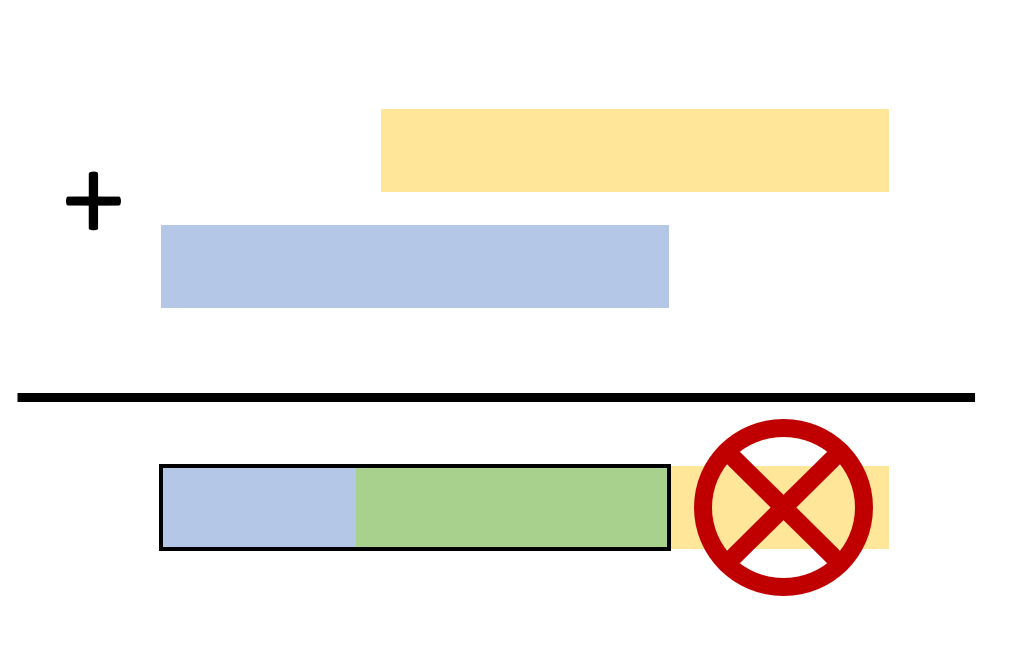
\includegraphics[width=0.5\textwidth]{addition}
      \errorcomputing
      \end{center}
        \end{frame}
        
  \begin{frame}{En C++}
    Dans la STL :
    \begin{itemize}
    \item numeric\textunderscore limits (min, max, lowest, round\textunderscore error, epsilon, ...)
    \item nextafter (permet de calculer l'ULP)
    \item isnan, isinf, ...
    \item frexp, ldexp, logb, ...
    \item gestion des environnements (exceptions, arrondis)
    \end{itemize}
  \end{frame}
  
    \begin{frame}{Solutions 1/N}
  Utiliser des doubles au lieu de floats, voir des quadruples sur des architectures qui le permettent. \\
  Inconvénients :
  \begin{itemize}
  \item Réécriture ou modifications de codes sources
  \item Perte importante de performance (bande passante)
  \item Pas de certitude quant à la validité/stabilité des résultats
  \end{itemize} 
  \end{frame}
  
  \begin{frame}{Recherche}
La stabilité numérique est un champ de recherche à lui seul. Pour les analyses, plusieurs méthodes existent : 
\begin{itemize}
\item Stochastique des arrondis (arrondis aléatoires sur les opérations)
\item Calcul d'intervalles (opérations sur les arrondis et troncatures, puis min/max de chaque)
\item Propagation d'erreurs (calcul des rests d'arrondis et propagation dans le code)
\end{itemize}
  \end{frame}
  
    \begin{frame}{Outil : CADNA}
    \begin{itemize}
    \item Modification/adaptation des fichiers sources
    \item Calcul du nombre de chiffres significatifs
    \item Lors de chaque opération, on calcul l'erreur d'arrondi
    \item Cibles : CPU, GPU, vectorisé, MPI, OpenMP
    \item CADTRACE : Analyse et identification automatique des opérations les plus instables
    \end{itemize}
  \end{frame}
  
\defverbatim[colored]\cadnanosample{
\begin{lstlisting}[language=C++,basicstyle=\ttfamily,keywordstyle=\color{blue}]
int main() {
  double x = 77617.;
  double y = 33096.;
  double res;

  res=333.75*pow(y, 6)+x*x*(11*x*x*y*y-pow(y, 5)
  -121*pow(y, 4)-2.0)+5.5*pow(y, 8)+x/(2*y);

  return 0;
}
\end{lstlisting}
}
  
  \begin{frame}{Outil : CADNA}
\cadnanosample
  \end{frame}
  
  \defverbatim[colored]\cadnasample{
\begin{lstlisting}[language=C++,basicstyle=\ttfamily,keywordstyle=\color{blue}]
int main()
{
  cadna_init(-1);
  double_st x = 77617.;
  double_st y = 33096.;
  double_st res;

  res=333.75*pow(y, 6)+x*x*(11*x*x*y*y-pow(y, 5)
  -121*pow(y, 4)-2.0)+5.5*pow(y, 8)+x/(2*y);

  cadna_end();
}
\end{lstlisting}
}

    \begin{frame}{Outil : CADNA}
\cadnasample
  \end{frame}
  
    \begin{frame}{Outil : PROMISE}
        \begin{itemize}
    \item Utilise CADNA
    \item "Autotune" du flottant
    \item Nécessite de modifier les sources pour remplacer les types par des balises qui seront surchargées lors de la compilation
    \item Très pertinent dans le cadre de recherche de performances
    \item Besoin de fixer des variables/critères d'acceptation
    \item Test sur le nombre de chiffres significatifs
    \end{itemize}
  \end{frame}

  
      \begin{frame}{Outil : Verificarlo}
\begin{itemize}
\item Chaine de compilation (basé sur LLVM)
\item Pas de modification de code sources, mais recompilation
\item Remplacement des types float, double par des types externes
\item Possibilité d'utiliser plusieurs backends lors de l'exécution du programme (shared lib) : IEEE, modes d'arrondi, arrondi aléatoire, valeur arbitraire de précision, détection d'annulation, modification du format IEEE-754
\end{itemize}
  \end{frame}
    
      
    \begin{frame}{Outil : Verrou/Padlock}
\begin{itemize}
\item Plugin Valgrind
\item Utilisation de l'exécutable directement
\item Choix du type d'arrondi
\item Plusieurs runs permettent d'avoir une vue précise de la stabilité du programme
\item Impact très important sur le temps d'exécution
\end{itemize}
  \end{frame}
    
  \begin{frame}{Valeurs particulières : nombre dénormalisé}
  Pour les valeurs proches de 0.0, ie avec un exposant nul (équivalent à $2^{-127}$)
  \begin{itemize}
  \item 0b \textcolor{SignColor}{y} \textcolor{ExponentColor}{00000000} \textcolor{FractionColor}{xxxxxxxxxxxxxxxxxxxxxxx}
  \item Suppression de la troncature du premier bit et l'exposant a pour valeur -126 pour assurer la continuité 
  \item La plus petite valeur représentable est ainsi $1.40129846432*10^{-45}$ au lieu de $1.17549435*10^{-38}$
  \end{itemize}

  \end{frame}

  \begin{frame}{Valeur particulière : -0.0}
    \begin{large}
  2 valeurs de zéro dans les nombres flottants :
  \begin{itemize}
  \item 0.0 $\Rightarrow$ 0b \textcolor{SignColor}{0} \textcolor{ExponentColor}{00000000} \textcolor{FractionColor}{00000000000000000000000} \\
  \item -0.0 $\Rightarrow$ 0b \textcolor{SignColor}{1} \textcolor{ExponentColor}{00000000} \textcolor{FractionColor}{00000000000000000000000}
  \end{itemize}
        \end{large}
  \end{frame}

  \begin{frame}{Valeurs particulières : +/- Inf}
      \begin{large}
  2 valeurs d'infini pour les nombres flottants :
  \begin{itemize}
  \item $\infty \Rightarrow$ 0b \textcolor{SignColor}{0} \textcolor{ExponentColor}{11111111} \textcolor{FractionColor}{00000000000000000000000} \\
    \item $-\infty \Rightarrow$ 0b \textcolor{SignColor}{1} \textcolor{ExponentColor}{11111111} \textcolor{FractionColor}{00000000000000000000000} \\
  \end{itemize}
        \end{large}
  \end{frame}
  
  \begin{frame}{Valeurs particulières : NaN}
      \begin{large}
  NaNs (Not a Number), $2^{1+size(mantisse)}$ valeurs possibles :
  \begin{itemize}
  \item Résultat d'un calcul invalide, overflow, ...
  \item 0b \textcolor{SignColor}{y} \textcolor{ExponentColor}{11111111} \textcolor{FractionColor}{xxxxxxxxxxxxxxxxxxxxxxx} (avec au moins un x à 1)\\
  \item inf est un NaN
  \item Certains code de calcul utilise la mantisse comme payload $\Rightarrow$ attention à l'utilisation des outils ci-dessus
  \end{itemize}
        \end{large}
  \end{frame}

  \begin{frame}{Points non abordés}
  \begin{itemize}
  \item Delta debug
  \item Le reste de la norme IEEE-754 et ses évolutions 2008 et 2019
  \item Autres représentations (Unum, bfloat, fixed precision, big decimal, ...)
  \item Impact des FPU
  \item Extended precision
  \end{itemize}
  \end{frame}

  \begin{frame}{Liens utiles}
  \begin{itemize}
  \item Convertisseur FP : https://www.h-schmidt.net/FloatConverter/IEEE754.html
  \item InterFLOP : https://calcul.math.cnrs.fr/attachments/evt/2019-06-precision-num/support04.pdf
  \item CADNA : http://cadna.lip6.fr/
  \end{itemize}
  \end{frame}

\end{document}
